\documentclass[a4paper]{book}
\usepackage{a4wide}
\usepackage{makeidx}
\usepackage{graphicx}
\usepackage{multicol}
\usepackage{float}
\usepackage{listings}
\usepackage{color}
\usepackage{textcomp}
\usepackage{alltt}
\usepackage{times}
\usepackage{ifpdf}
\ifpdf
\usepackage[pdftex,
            pagebackref=true,
            colorlinks=true,
            linkcolor=blue,
            unicode
           ]{hyperref}
\else
\usepackage[ps2pdf,
            pagebackref=true,
            colorlinks=true,
            linkcolor=blue,
            unicode
           ]{hyperref}
\usepackage{pspicture}
\fi
\usepackage[utf8]{inputenc}
\usepackage[french]{babel}

\usepackage{doxygen}
\lstset{language=C++,inputencoding=utf8,basicstyle=\footnotesize,breaklines=true,breakatwhitespace=true,tabsize=2,numbers=left }
\makeindex
\setcounter{tocdepth}{3}
\renewcommand{\footrulewidth}{0.4pt}
\begin{document}
\hypersetup{pageanchor=false}
\begin{titlepage}
\vspace*{7cm}
\begin{center}
{\Large Exemple de documentation avec Doxygen \\[1ex]\large 1 }\\
\vspace*{1cm}
{\large Généré par Doxygen 1.6.1}\\
\vspace*{0.5cm}
{\small Sun Sep 27 18:14:27 2009}\\
\end{center}
\end{titlepage}
\clearemptydoublepage
\pagenumbering{roman}
\tableofcontents
\clearemptydoublepage
\pagenumbering{arabic}
\hypersetup{pageanchor=true}
\chapter{Ma page d'introduction perso}
\label{index}\hypertarget{index}{}Ceci est l'introduction du document.  
\chapter{Liste des choses à faire}
\label{todo}
\hypertarget{todo}{}
\label{todo__todo000001}
\hypertarget{todo__todo000001}{}
 
\begin{DoxyDescription}
\item[Membre \hyperlink{class_class_b_ac17b7f1214a74505d7882ebf9ddcb65e}{ClassB::maMethode}() ]Ecrire un code fonctionnel. 
\end{DoxyDescription}
\chapter{Liste des éléments obsolètes}
\label{deprecated}
\hypertarget{deprecated}{}
\label{deprecated__deprecated000001}
\hypertarget{deprecated__deprecated000001}{}
 
\begin{DoxyDescription}
\item[Membre \hyperlink{class_class_a_aa95d318339e8bdb65954c7942f1e1f78}{ClassA::maMethode}() ]Ne pas l'utiliser sinon plantage assuré... 
\end{DoxyDescription}
\chapter{Liste des bogues}
\label{bug}
\hypertarget{bug}{}
\label{bug__bug000001}
\hypertarget{bug__bug000001}{}
 
\begin{DoxyDescription}
\item[Membre \hyperlink{class_class_a_aa95d318339e8bdb65954c7942f1e1f78}{ClassA::maMethode}() ]BSOD 
\end{DoxyDescription}
\chapter{Index des classes}
\section{Liste des classes}
Liste des classes, structures, unions et interfaces avec une brève description :\begin{DoxyCompactList}
\item\contentsline{section}{\hyperlink{class_class_a}{ClassA} (Classe d'exemple A )}{\pageref{class_class_a}}{}
\item\contentsline{section}{\hyperlink{class_class_b}{ClassB} (Classe d'exemple B )}{\pageref{class_class_b}}{}
\item\contentsline{section}{\hyperlink{struct_class_a_1_1_ma_struct}{ClassA::MaStruct} (Ma structure interne )}{\pageref{struct_class_a_1_1_ma_struct}}{}
\end{DoxyCompactList}

\chapter{Index des fichiers}
\section{Liste des fichiers}
Liste de tous les fichiers avec une brève description :\begin{DoxyCompactList}
\item\contentsline{section}{\hyperlink{_class_a_8cpp}{ClassA.cpp} }{\pageref{_class_a_8cpp}}{}
\item\contentsline{section}{\hyperlink{_class_a_8hpp}{ClassA.hpp} }{\pageref{_class_a_8hpp}}{}
\item\contentsline{section}{\hyperlink{_class_b_8cpp}{ClassB.cpp} }{\pageref{_class_b_8cpp}}{}
\item\contentsline{section}{\hyperlink{_class_b_8hpp}{ClassB.hpp} }{\pageref{_class_b_8hpp}}{}
\end{DoxyCompactList}

\chapter{Documentation des classes}
\hypertarget{class_class_a}{
\section{Référence de la classe ClassA}
\label{class_class_a}\index{ClassA@{ClassA}}
}


Classe d'exemple A.  


{\ttfamily \#include $<$ClassA.hpp$>$}Graphe de collaboration de ClassA:\nopagebreak
\begin{figure}[H]
\begin{center}
\leavevmode
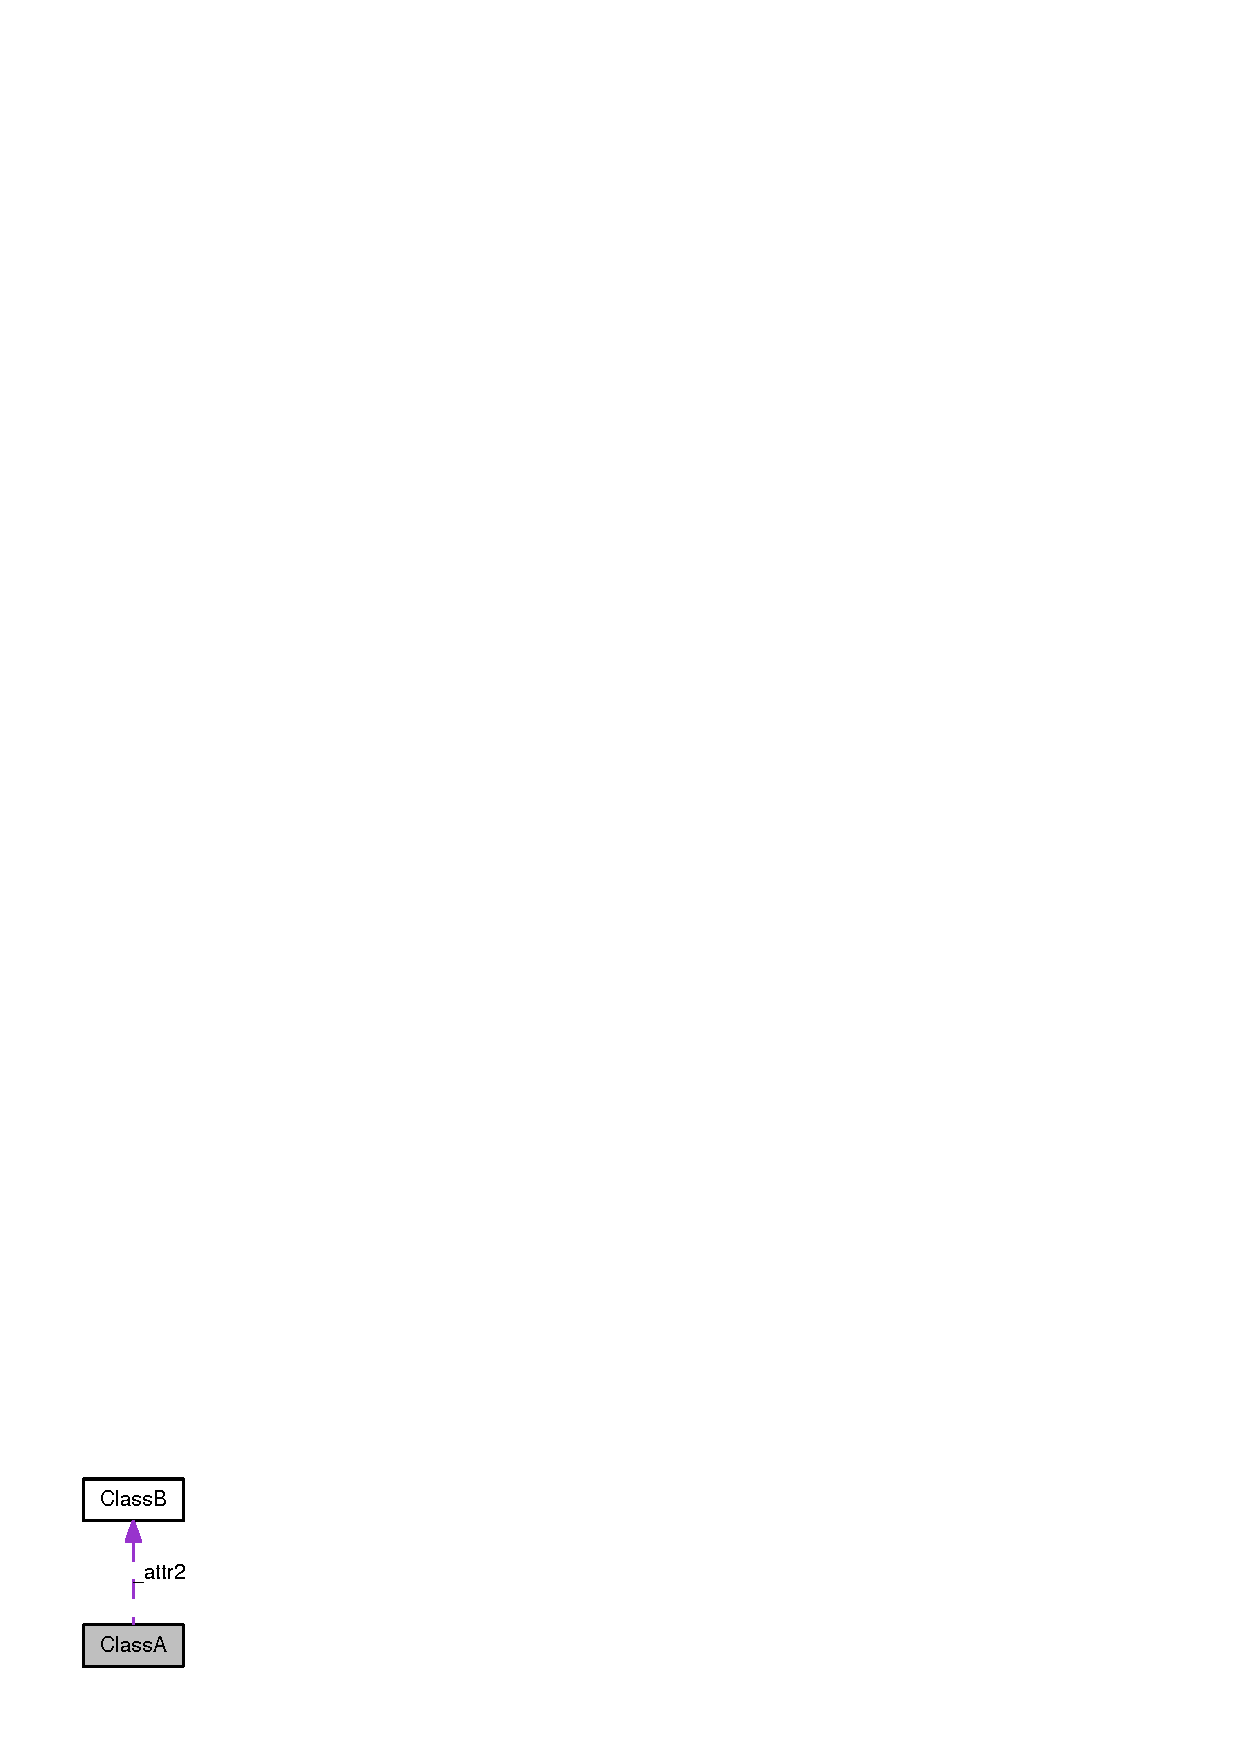
\includegraphics[width=93pt]{class_class_a__coll__graph}
\end{center}
\end{figure}
\subsection*{Classes}
\begin{DoxyCompactItemize}
\item 
struct \hyperlink{struct_class_a_1_1_ma_struct}{MaStruct}
\begin{DoxyCompactList}\small\item\em Ma structure interne. \item\end{DoxyCompactList}\end{DoxyCompactItemize}
\subsection*{Fonctions membres publiques}
\begin{DoxyCompactItemize}
\item 
\hyperlink{class_class_a_acd165fa87ae77eeb9c715024c0301a6b}{ClassA} ()
\begin{DoxyCompactList}\small\item\em Constructeur par défaut. \item\end{DoxyCompactList}\item 
\hyperlink{class_class_a_a6ead4513f775571caf3c0387d535783f}{$\sim$ClassA} ()
\begin{DoxyCompactList}\small\item\em Destructeur par défaut. \item\end{DoxyCompactList}\item 
\hyperlink{struct_class_a_1_1_ma_struct}{MaStruct} $\ast$ \hyperlink{class_class_a_aa95d318339e8bdb65954c7942f1e1f78}{maMethode} ()
\begin{DoxyCompactList}\small\item\em Ma méthode, et à personne d'autre ! \item\end{DoxyCompactList}\item 
\hyperlink{struct_class_a_1_1_ma_struct}{MaStruct} $\ast$ \hyperlink{class_class_a_a30a91a34f55c7cafb8922c55c0e99d50}{maMethode} (int param1, const string param2)
\begin{DoxyCompactList}\small\item\em Version améliorée de ma méthode, et à personne d'autre ! \item\end{DoxyCompactList}\end{DoxyCompactItemize}
\subsection*{Types privés}
\begin{DoxyCompactItemize}
\item 
enum \hyperlink{class_class_a_aebd12939da3b00aca5f7c04a0f34f0d4}{MonEnum} \{ \hyperlink{class_class_a_aebd12939da3b00aca5f7c04a0f34f0d4a9db1f0ab44af74bb349827f67c63835d}{VAL1} =  1, 
\hyperlink{class_class_a_aebd12939da3b00aca5f7c04a0f34f0d4a2aa208680503684c42107f008350be56}{VAL2} =  10, 
\hyperlink{class_class_a_aebd12939da3b00aca5f7c04a0f34f0d4ab9438dfedb4070dba86d8dfaf4562851}{VAL3} =  100
 \}
\begin{DoxyCompactList}\small\item\em Une énumération de trois valeurs sur une échelle logarithmique 10. \item\end{DoxyCompactList}\end{DoxyCompactItemize}
\subsection*{Attributs privés}
\begin{DoxyCompactItemize}
\item 
long int \hyperlink{class_class_a_ab13fa04135597d1b015171ee7e823804}{\_\-attr1}
\begin{DoxyCompactList}\small\item\em Mon premier attribut. \item\end{DoxyCompactList}\item 
\hyperlink{class_class_b}{ClassB} $\ast$ \hyperlink{class_class_a_a705a48160d35a8656f1196967a3f11ab}{\_\-attr2}
\begin{DoxyCompactList}\small\item\em Mon second attribut : pointeur vers instance de B. \item\end{DoxyCompactList}\end{DoxyCompactItemize}
\subsection*{Attributs privés statiques}
\begin{DoxyCompactItemize}
\item 
static const \hyperlink{class_class_a_a37b03b75edb033b486bdbaeb5019cc08}{THE\_\-ANSWER} = 40 + 2
\begin{DoxyCompactList}\small\item\em Constante de classe répondant à la grande question sur l'Univers. \item\end{DoxyCompactList}\end{DoxyCompactItemize}


\subsection{Description détaillée}
Classe d'exemple A. Voici un petit bout de code qui illustre l'utilisation de Doxygen au travers d'un code de classe C++. \begin{DoxyAuthor}{Auteur}
Emmanuel GAUDE $<$\href{mailto:emmanuel.gaude@etu.univ-lyon1.fr}{\tt emmanuel.gaude@etu.univ-\/lyon1.fr}$>$ 

Benjamin GUILLON $<$\href{mailto:benjamin.guillon@etu.univ-lyon1.fr}{\tt benjamin.guillon@etu.univ-\/lyon1.fr}$>$ 
\end{DoxyAuthor}
\begin{DoxySince}{Depuis}
2009/09/26 
\end{DoxySince}
\begin{DoxyVersion}{Version}
2009/10/03
\end{DoxyVersion}
\begin{DoxySeeAlso}{Voir également}
\href{http://www.stack.nl/~dimitri/doxygen/manual.html}{\tt http://www.stack.nl/$\sim$dimitri/doxygen/manual.html} 
\end{DoxySeeAlso}
\begin{DoxyNote}{Note}
Vous mettez ici ce que vous voulez, comme une licence. 
\end{DoxyNote}


\subsection{Documentation des énumérations membres}
\hypertarget{class_class_a_aebd12939da3b00aca5f7c04a0f34f0d4}{
\index{ClassA@{ClassA}!MonEnum@{MonEnum}}
\index{MonEnum@{MonEnum}!ClassA@{ClassA}}
\subsubsection[{MonEnum}]{\setlength{\rightskip}{0pt plus 5cm}enum {\bf ClassA::MonEnum}\hspace{0.3cm}{\ttfamily  \mbox{[}private\mbox{]}}}}
\label{class_class_a_aebd12939da3b00aca5f7c04a0f34f0d4}


Une énumération de trois valeurs sur une échelle logarithmique 10. \begin{Desc}
\item[Valeurs énumérées: ]\par
\begin{description}
\index{VAL1@{VAL1}!ClassA@{ClassA}}\index{ClassA@{ClassA}!VAL1@{VAL1}}\item[{\em 
\hypertarget{class_class_a_aebd12939da3b00aca5f7c04a0f34f0d4a9db1f0ab44af74bb349827f67c63835d}{
VAL1}
\label{class_class_a_aebd12939da3b00aca5f7c04a0f34f0d4a9db1f0ab44af74bb349827f67c63835d}
}]Première valeur de l'énum (1) \index{VAL2@{VAL2}!ClassA@{ClassA}}\index{ClassA@{ClassA}!VAL2@{VAL2}}\item[{\em 
\hypertarget{class_class_a_aebd12939da3b00aca5f7c04a0f34f0d4a2aa208680503684c42107f008350be56}{
VAL2}
\label{class_class_a_aebd12939da3b00aca5f7c04a0f34f0d4a2aa208680503684c42107f008350be56}
}]Deuxième valeur de l'énum (10) \index{VAL3@{VAL3}!ClassA@{ClassA}}\index{ClassA@{ClassA}!VAL3@{VAL3}}\item[{\em 
\hypertarget{class_class_a_aebd12939da3b00aca5f7c04a0f34f0d4ab9438dfedb4070dba86d8dfaf4562851}{
VAL3}
\label{class_class_a_aebd12939da3b00aca5f7c04a0f34f0d4ab9438dfedb4070dba86d8dfaf4562851}
}]Troisième valeur de l'énum (100) \end{description}
\end{Desc}



\subsection{Documentation des constructeurs et destructeur}
\hypertarget{class_class_a_acd165fa87ae77eeb9c715024c0301a6b}{
\index{ClassA@{ClassA}!ClassA@{ClassA}}
\index{ClassA@{ClassA}!ClassA@{ClassA}}
\subsubsection[{ClassA}]{\setlength{\rightskip}{0pt plus 5cm}ClassA::ClassA ()}}
\label{class_class_a_acd165fa87ae77eeb9c715024c0301a6b}


Constructeur par défaut. Classe d'exemple A \hypertarget{class_class_a_a6ead4513f775571caf3c0387d535783f}{
\index{ClassA@{ClassA}!$\sim$ClassA@{$\sim$ClassA}}
\index{$\sim$ClassA@{$\sim$ClassA}!ClassA@{ClassA}}
\subsubsection[{$\sim$ClassA}]{\setlength{\rightskip}{0pt plus 5cm}ClassA::$\sim$ClassA ()}}
\label{class_class_a_a6ead4513f775571caf3c0387d535783f}


Destructeur par défaut. 

\subsection{Documentation des fonctions membres}
\hypertarget{class_class_a_a30a91a34f55c7cafb8922c55c0e99d50}{
\index{ClassA@{ClassA}!maMethode@{maMethode}}
\index{maMethode@{maMethode}!ClassA@{ClassA}}
\subsubsection[{maMethode}]{\setlength{\rightskip}{0pt plus 5cm}double ClassA::maMethode (int {\em param1}, \/  const string {\em param2})}}
\label{class_class_a_a30a91a34f55c7cafb8922c55c0e99d50}


Version améliorée de ma méthode, et à personne d'autre ! 
\begin{DoxyParams}{Paramètres}
\item[\mbox{$\leftrightarrow$} {\em param1}]Entier dont il faut calculer la racine carrée. \item[\mbox{$\leftarrow$} {\em param2}]Message à afficher. \end{DoxyParams}
\begin{DoxyReturn}{Renvoie}
Retourne un pointeur sur un nouvel objet \hyperlink{struct_class_a_1_1_ma_struct}{MaStruct} initialisé avec param1. 
\end{DoxyReturn}
\hypertarget{class_class_a_aa95d318339e8bdb65954c7942f1e1f78}{
\index{ClassA@{ClassA}!maMethode@{maMethode}}
\index{maMethode@{maMethode}!ClassA@{ClassA}}
\subsubsection[{maMethode}]{\setlength{\rightskip}{0pt plus 5cm}double ClassA::maMethode ()}}
\label{class_class_a_aa95d318339e8bdb65954c7942f1e1f78}


Ma méthode, et à personne d'autre ! \begin{DoxyPrecond}{Précondition}
Un système sous Windows... 
\end{DoxyPrecond}
\begin{DoxyPostcond}{Postcondition}
Une perte de données.
\end{DoxyPostcond}
\begin{DoxyReturn}{Renvoie}
Retourne systématiquement NULL. 
\end{DoxyReturn}
\begin{Desc}
\item[\hyperlink{deprecated__deprecated000001}{Obsolète}]Ne pas l'utiliser sinon plantage assuré... \end{Desc}
\begin{Desc}
\item[\hyperlink{bug__bug000001}{Bogue}]BSOD \end{Desc}


\subsection{Documentation des données membres}
\hypertarget{class_class_a_ab13fa04135597d1b015171ee7e823804}{
\index{ClassA@{ClassA}!\_\-attr1@{\_\-attr1}}
\index{\_\-attr1@{\_\-attr1}!ClassA@{ClassA}}
\subsubsection[{\_\-attr1}]{\setlength{\rightskip}{0pt plus 5cm}long int {\bf ClassA::\_\-attr1}\hspace{0.3cm}{\ttfamily  \mbox{[}private\mbox{]}}}}
\label{class_class_a_ab13fa04135597d1b015171ee7e823804}


Mon premier attribut. \hypertarget{class_class_a_a705a48160d35a8656f1196967a3f11ab}{
\index{ClassA@{ClassA}!\_\-attr2@{\_\-attr2}}
\index{\_\-attr2@{\_\-attr2}!ClassA@{ClassA}}
\subsubsection[{\_\-attr2}]{\setlength{\rightskip}{0pt plus 5cm}{\bf ClassB}$\ast$ {\bf ClassA::\_\-attr2}\hspace{0.3cm}{\ttfamily  \mbox{[}private\mbox{]}}}}
\label{class_class_a_a705a48160d35a8656f1196967a3f11ab}


Mon second attribut : pointeur vers instance de B. \hypertarget{class_class_a_a37b03b75edb033b486bdbaeb5019cc08}{
\index{ClassA@{ClassA}!THE\_\-ANSWER@{THE\_\-ANSWER}}
\index{THE\_\-ANSWER@{THE\_\-ANSWER}!ClassA@{ClassA}}
\subsubsection[{THE\_\-ANSWER}]{\setlength{\rightskip}{0pt plus 5cm}const {\bf ClassA::THE\_\-ANSWER} = 40 + 2\hspace{0.3cm}{\ttfamily  \mbox{[}static, private\mbox{]}}}}
\label{class_class_a_a37b03b75edb033b486bdbaeb5019cc08}


Constante de classe répondant à la grande question sur l'Univers. 

La documentation de cette classe a été générée à partir des fichiers suivants :\begin{DoxyCompactItemize}
\item 
\hyperlink{_class_a_8hpp}{ClassA.hpp}\item 
\hyperlink{_class_a_8cpp}{ClassA.cpp}\end{DoxyCompactItemize}

\hypertarget{class_class_b}{
\section{Référence de la classe ClassB}
\label{class_class_b}\index{ClassB@{ClassB}}
}


Classe d'exemple B.  


{\ttfamily \#include $<$ClassB.hpp$>$}\subsection*{Fonctions membres publiques}
\begin{DoxyCompactItemize}
\item 
\hyperlink{class_class_b_a327bbcde6f569ee4d180d82aa894605e}{ClassB} (const string monNom)
\begin{DoxyCompactList}\small\item\em Constructeur de la classe. \item\end{DoxyCompactList}\item 
string \hyperlink{class_class_b_a52a89bf5f66d82ae413610aea58363ca}{getMonNom} () const 
\begin{DoxyCompactList}\small\item\em Accesseur de \_\-monNom. \item\end{DoxyCompactList}\item 
void \hyperlink{class_class_b_a8294ff99ed4904787e47ca15f07e2ace}{setMonNom} (string monNom)
\begin{DoxyCompactList}\small\item\em Modificateur de \_\-monNom. \item\end{DoxyCompactList}\item 
double \hyperlink{class_class_b_ac17b7f1214a74505d7882ebf9ddcb65e}{maMethode} ()
\begin{DoxyCompactList}\small\item\em Ma méthode. \item\end{DoxyCompactList}\end{DoxyCompactItemize}
\subsection*{Attributs privés}
\begin{DoxyCompactItemize}
\item 
string \hyperlink{class_class_b_a1014a29d4201c63e8ebd40c027eb2fc7}{\_\-monNom}
\begin{DoxyCompactList}\small\item\em Nom de l'instance. \item\end{DoxyCompactList}\end{DoxyCompactItemize}


\subsection{Description détaillée}
Classe d'exemple B. \begin{DoxySince}{Depuis}
2009/09/26 
\end{DoxySince}
\begin{DoxyVersion}{Version}
2009/10/03
\end{DoxyVersion}
Une autre classe plus succinte pour compléter la classe A. \begin{DoxyAuthor}{Auteur}
Emmanuel GAUDE $<$\href{mailto:emmanuel.gaude@etu.univ-lyon1.fr}{\tt emmanuel.gaude@etu.univ-\/lyon1.fr}$>$ 

Benjamin GUILLON $<$\href{mailto:benjamin.guillon@etu.univ-lyon1.fr}{\tt benjamin.guillon@etu.univ-\/lyon1.fr}$>$
\end{DoxyAuthor}
\begin{DoxySeeAlso}{Voir également}
\href{http://www.stack.nl/~dimitri/doxygen/manual.html}{\tt http://www.stack.nl/$\sim$dimitri/doxygen/manual.html} 
\end{DoxySeeAlso}
\begin{DoxyNote}{Note}
Vous mettez ici ce que vous voulez, comme une licence. 
\end{DoxyNote}


\subsection{Documentation des constructeurs et destructeur}
\hypertarget{class_class_b_a327bbcde6f569ee4d180d82aa894605e}{
\index{ClassB@{ClassB}!ClassB@{ClassB}}
\index{ClassB@{ClassB}!ClassB@{ClassB}}
\subsubsection[{ClassB}]{\setlength{\rightskip}{0pt plus 5cm}ClassB::ClassB (const string {\em monNom})}}
\label{class_class_b_a327bbcde6f569ee4d180d82aa894605e}


Constructeur de la classe. \begin{DoxyPrecond}{Précondition}
monNom non vide. 
\end{DoxyPrecond}
\begin{DoxyPostcond}{Postcondition}
Construit un objet de type \hyperlink{class_class_b}{ClassB}.
\end{DoxyPostcond}

\begin{DoxyParams}{Paramètres}
\item[\mbox{$\leftarrow$} {\em monNom}]Nom de l'instance.\end{DoxyParams}

\begin{DoxyExceptions}{Exceptions}
\item[{\em Exception}]Retourne une exception de type Exception si monNom est vide.\end{DoxyExceptions}
Classe d'exemple B 

\subsection{Documentation des fonctions membres}
\hypertarget{class_class_b_a52a89bf5f66d82ae413610aea58363ca}{
\index{ClassB@{ClassB}!getMonNom@{getMonNom}}
\index{getMonNom@{getMonNom}!ClassB@{ClassB}}
\subsubsection[{getMonNom}]{\setlength{\rightskip}{0pt plus 5cm}string ClassB::getMonNom () const}}
\label{class_class_b_a52a89bf5f66d82ae413610aea58363ca}


Accesseur de \_\-monNom. \begin{DoxyReturn}{Renvoie}
Nom de l'instance. 
\end{DoxyReturn}
\hypertarget{class_class_b_ac17b7f1214a74505d7882ebf9ddcb65e}{
\index{ClassB@{ClassB}!maMethode@{maMethode}}
\index{maMethode@{maMethode}!ClassB@{ClassB}}
\subsubsection[{maMethode}]{\setlength{\rightskip}{0pt plus 5cm}double ClassB::maMethode ()}}
\label{class_class_b_ac17b7f1214a74505d7882ebf9ddcb65e}


Ma méthode. \begin{DoxyReturn}{Renvoie}
Retourne systématiquement NULL. 
\end{DoxyReturn}

\begin{DoxyRetVals}{Valeurs retournées}
\item[{\em NULL}]Valeur normale de retour.\end{DoxyRetVals}
\begin{Desc}
\item[\hyperlink{todo__todo000001}{À faire}]Ecrire un code fonctionnel. \end{Desc}
\begin{DoxyWarning}{Avertissement}
La méthode de la classe A n'est pas la seule de ce nom finalement !
\end{DoxyWarning}

\begin{DoxyExceptions}{Exceptions}
\item[{\em Exception}]Retourne une exception si appelée une seconde fois. \end{DoxyExceptions}
\hypertarget{class_class_b_a8294ff99ed4904787e47ca15f07e2ace}{
\index{ClassB@{ClassB}!setMonNom@{setMonNom}}
\index{setMonNom@{setMonNom}!ClassB@{ClassB}}
\subsubsection[{setMonNom}]{\setlength{\rightskip}{0pt plus 5cm}void ClassB::setMonNom (string {\em monNom})}}
\label{class_class_b_a8294ff99ed4904787e47ca15f07e2ace}


Modificateur de \_\-monNom. 
\begin{DoxyParams}{Paramètres}
\item[\mbox{$\leftarrow$} {\em monNom}]Nom de l'instance.\end{DoxyParams}

\begin{DoxyExceptions}{Exceptions}
\item[{\em Exception}]Retourne une exception de type Exception si monNom est vide. \end{DoxyExceptions}


\subsection{Documentation des données membres}
\hypertarget{class_class_b_a1014a29d4201c63e8ebd40c027eb2fc7}{
\index{ClassB@{ClassB}!\_\-monNom@{\_\-monNom}}
\index{\_\-monNom@{\_\-monNom}!ClassB@{ClassB}}
\subsubsection[{\_\-monNom}]{\setlength{\rightskip}{0pt plus 5cm}string {\bf ClassB::\_\-monNom}\hspace{0.3cm}{\ttfamily  \mbox{[}private\mbox{]}}}}
\label{class_class_b_a1014a29d4201c63e8ebd40c027eb2fc7}


Nom de l'instance. 

La documentation de cette classe a été générée à partir des fichiers suivants :\begin{DoxyCompactItemize}
\item 
\hyperlink{_class_b_8hpp}{ClassB.hpp}\item 
\hyperlink{_class_b_8cpp}{ClassB.cpp}\end{DoxyCompactItemize}

\hypertarget{struct_class_a_1_1_ma_struct}{
\section{Référence de la structure ClassA::MaStruct}
\label{struct_class_a_1_1_ma_struct}\index{ClassA::MaStruct@{ClassA::MaStruct}}
}


Ma structure interne.  
\subsection*{Attributs publics}
\begin{DoxyCompactItemize}
\item 
int \hyperlink{struct_class_a_1_1_ma_struct_a3439feaf6316628cf77919d9f4b2519a}{attr1}
\begin{DoxyCompactList}\small\item\em Premier attribut de la structure. \item\end{DoxyCompactList}\item 
char \hyperlink{struct_class_a_1_1_ma_struct_aaaa68ea043748cccd75e3c0403ea4d87}{attr2}
\begin{DoxyCompactList}\small\item\em Second attribut de la structure. \item\end{DoxyCompactList}\end{DoxyCompactItemize}


\subsection{Description détaillée}
Ma structure interne. Une structure de données personnelle. 

\subsection{Documentation des données membres}
\hypertarget{struct_class_a_1_1_ma_struct_a3439feaf6316628cf77919d9f4b2519a}{
\index{ClassA::MaStruct@{ClassA::MaStruct}!attr1@{attr1}}
\index{attr1@{attr1}!ClassA::MaStruct@{ClassA::MaStruct}}
\subsubsection[{attr1}]{\setlength{\rightskip}{0pt plus 5cm}int {\bf ClassA::MaStruct::attr1}}}
\label{struct_class_a_1_1_ma_struct_a3439feaf6316628cf77919d9f4b2519a}


Premier attribut de la structure. \hypertarget{struct_class_a_1_1_ma_struct_aaaa68ea043748cccd75e3c0403ea4d87}{
\index{ClassA::MaStruct@{ClassA::MaStruct}!attr2@{attr2}}
\index{attr2@{attr2}!ClassA::MaStruct@{ClassA::MaStruct}}
\subsubsection[{attr2}]{\setlength{\rightskip}{0pt plus 5cm}char {\bf ClassA::MaStruct::attr2}}}
\label{struct_class_a_1_1_ma_struct_aaaa68ea043748cccd75e3c0403ea4d87}


Second attribut de la structure. 

La documentation de cette structure a été générée à partir du fichier suivant :\begin{DoxyCompactItemize}
\item 
\hyperlink{_class_a_8hpp}{ClassA.hpp}\end{DoxyCompactItemize}

\chapter{Documentation des fichiers}
\hypertarget{_class_a_8cpp}{
\section{Référence du fichier ClassA.cpp}
\label{_class_a_8cpp}\index{ClassA.cpp@{ClassA.cpp}}
}
{\ttfamily \#include \char`\"{}ClassA.hpp\char`\"{}}\par
Graphe des dépendances par inclusion de ClassA.cpp:\nopagebreak
\begin{figure}[H]
\begin{center}
\leavevmode
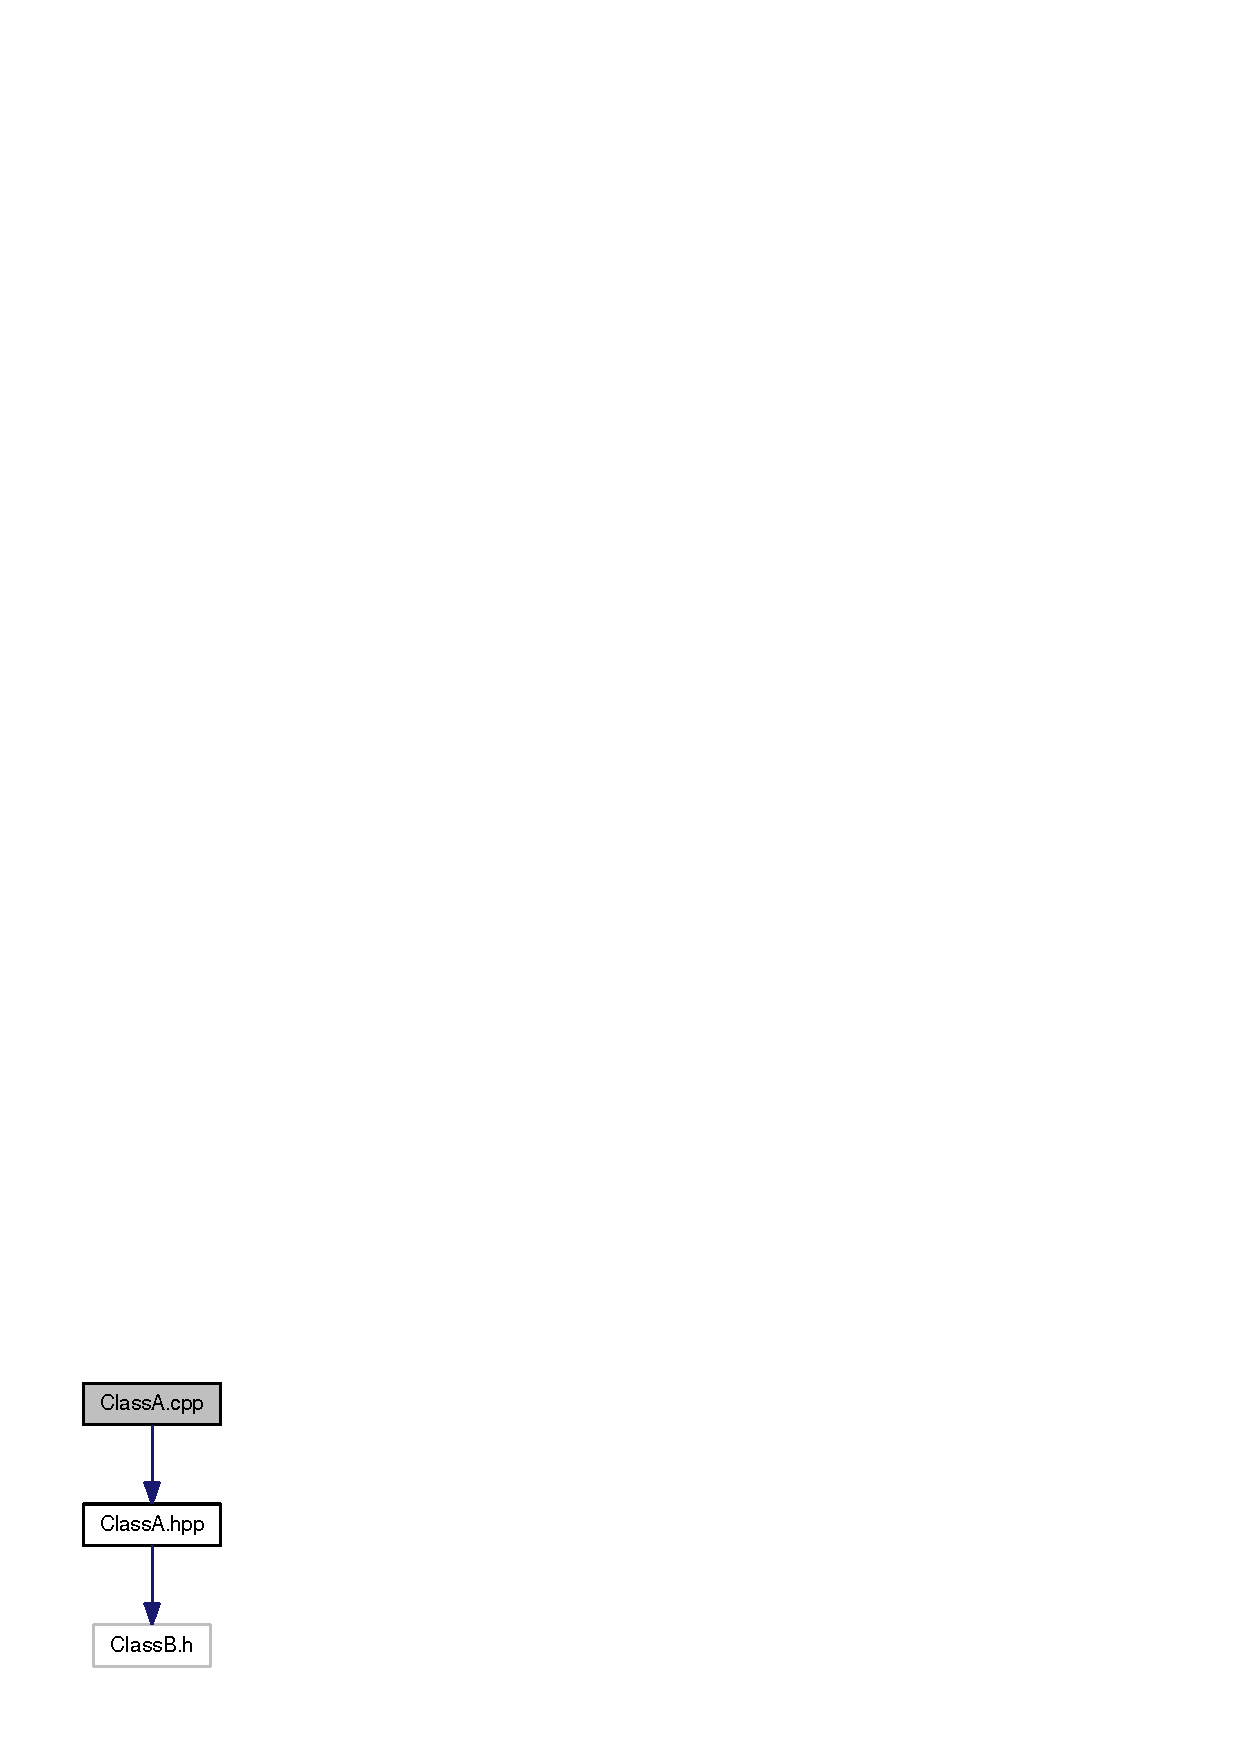
\includegraphics[width=55pt]{_class_a_8cpp__incl}
\end{center}
\end{figure}

\hypertarget{_class_a_8hpp}{
\section{Référence du fichier ClassA.hpp}
\label{_class_a_8hpp}\index{ClassA.hpp@{ClassA.hpp}}
}
{\ttfamily \#include \char`\"{}ClassB.h\char`\"{}}\par
Graphe des dépendances par inclusion de ClassA.hpp:\nopagebreak
\begin{figure}[H]
\begin{center}
\leavevmode
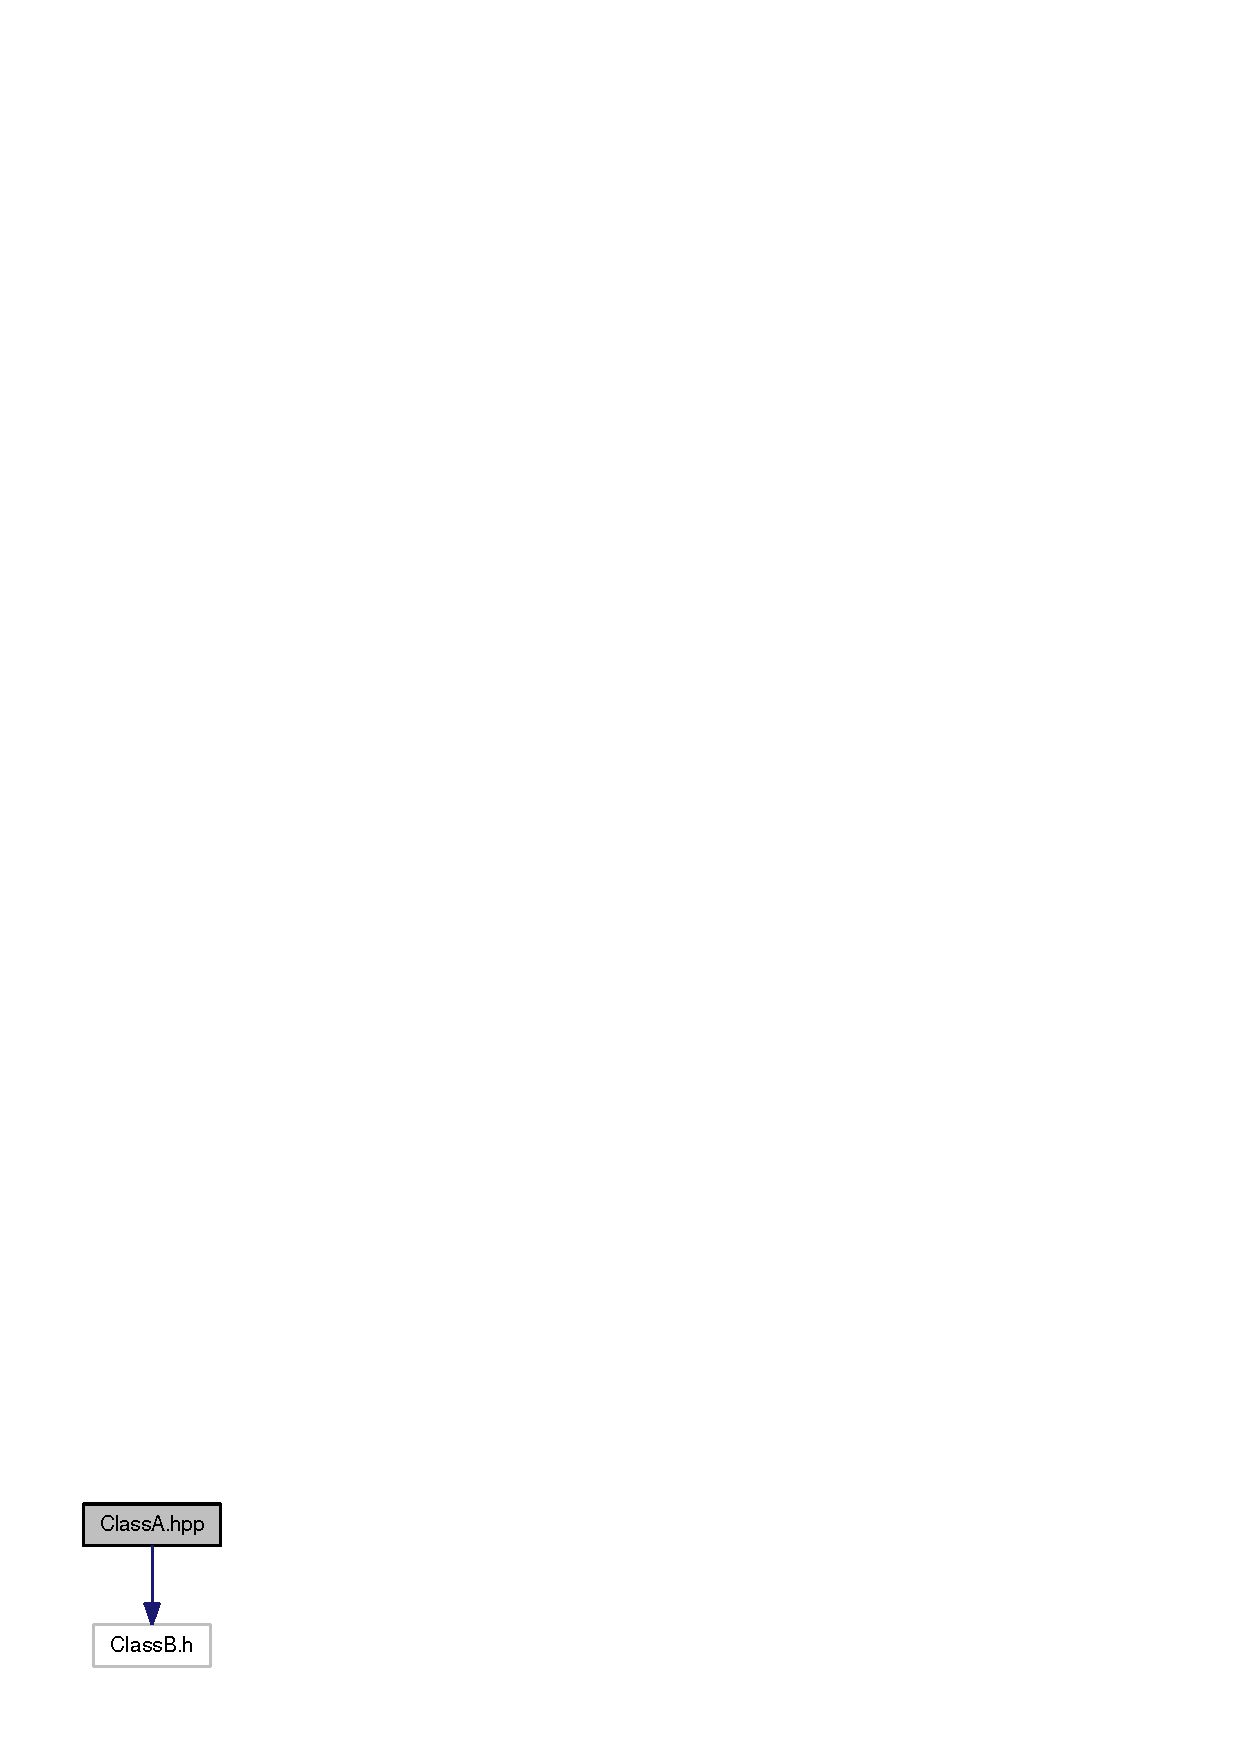
\includegraphics[width=55pt]{_class_a_8hpp__incl}
\end{center}
\end{figure}
Ce graphe montre quels fichiers incluent directement ou indirectement ce fichier :\nopagebreak
\begin{figure}[H]
\begin{center}
\leavevmode
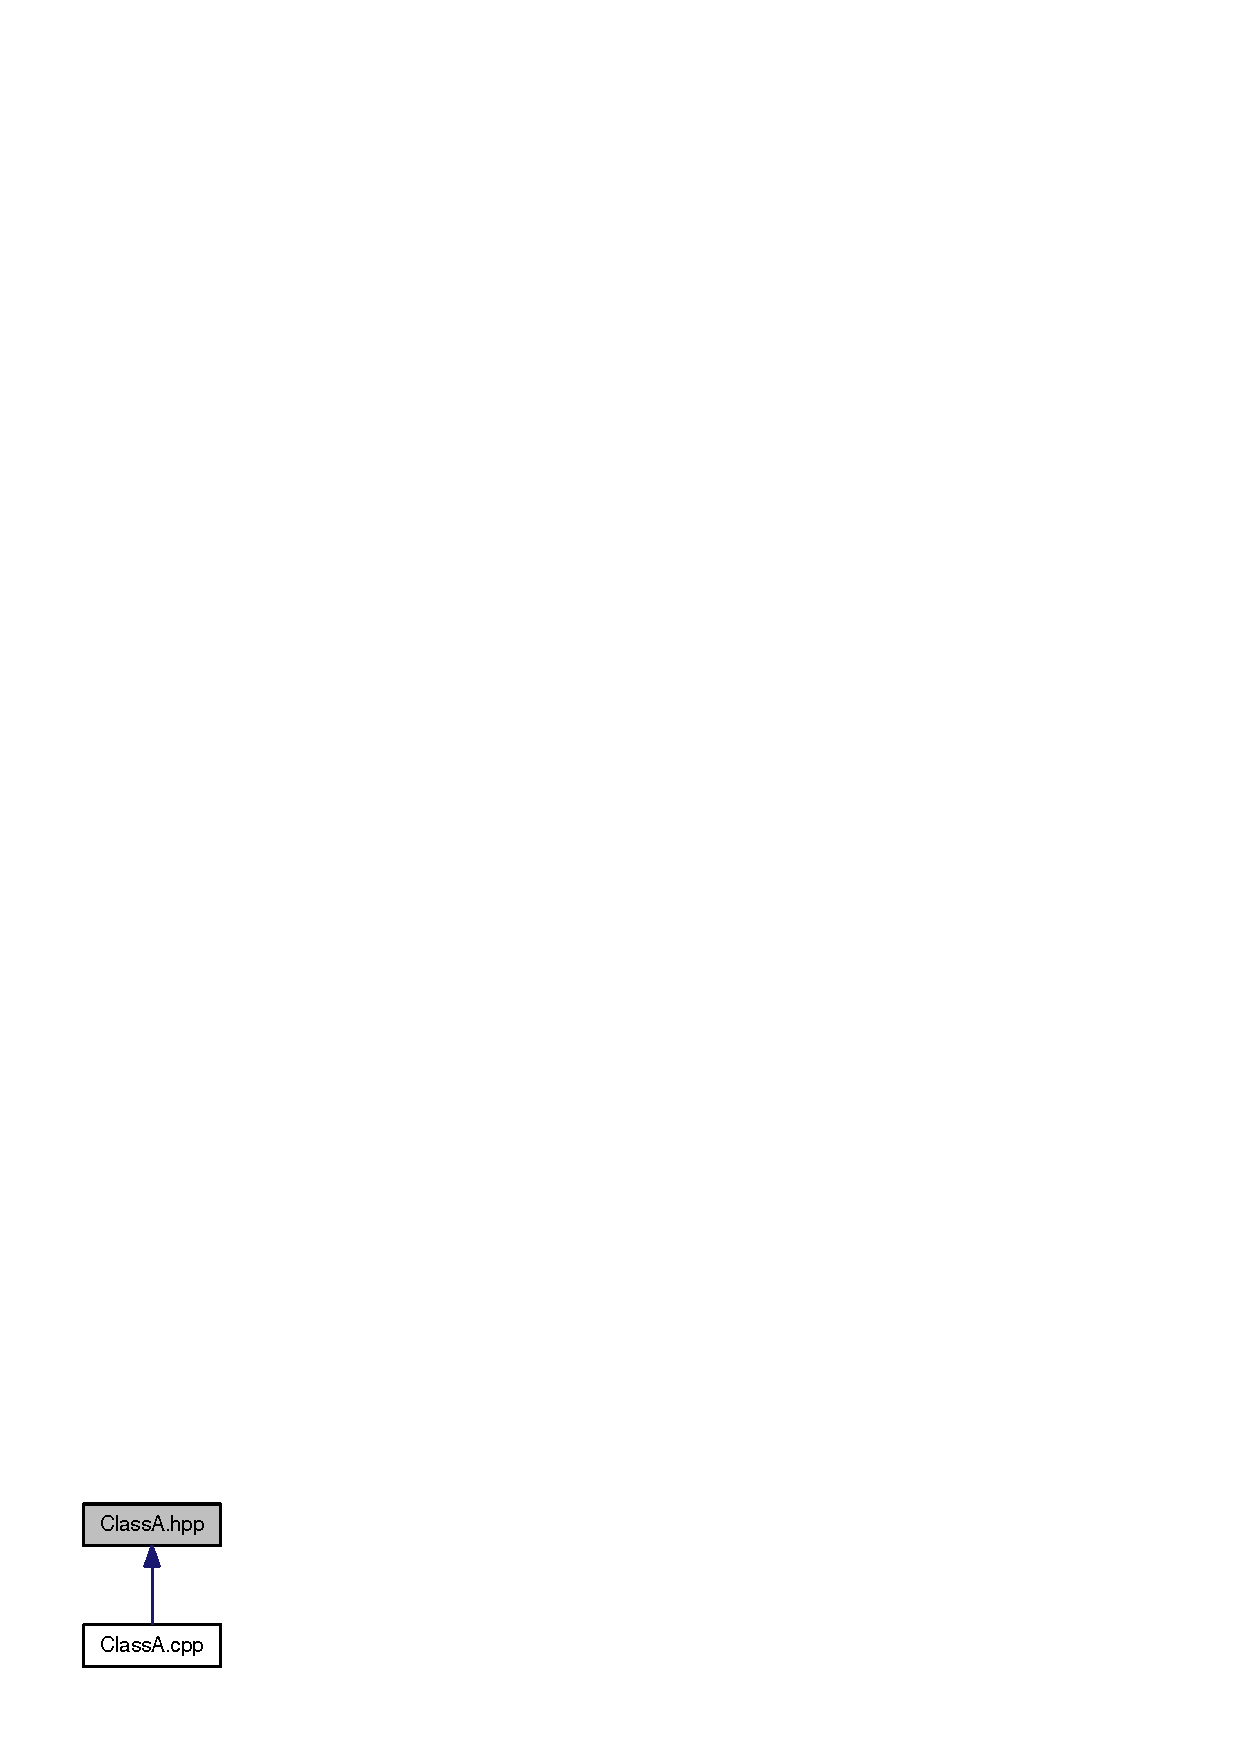
\includegraphics[width=55pt]{_class_a_8hpp__dep__incl}
\end{center}
\end{figure}
\subsection*{Classes}
\begin{DoxyCompactItemize}
\item 
class \hyperlink{class_class_a}{ClassA}
\begin{DoxyCompactList}\small\item\em Classe d'exemple A. \item\end{DoxyCompactList}\item 
struct \hyperlink{struct_class_a_1_1_ma_struct}{ClassA::MaStruct}
\begin{DoxyCompactList}\small\item\em Ma structure interne. \item\end{DoxyCompactList}\end{DoxyCompactItemize}
\subsection*{Macros}
\begin{DoxyCompactItemize}
\item 
\#define \hyperlink{_class_a_8hpp_a6af5917cc25c3507fffd8a94263575d9}{THE\_\-ANSWER\_\-MACRO}~40 + 2
\begin{DoxyCompactList}\small\item\em Macro calculant la valeur de La Réponse sur l'Univers. \item\end{DoxyCompactList}\end{DoxyCompactItemize}


\subsection{Description détaillée}


\subsection{Documentation des macros}
\hypertarget{_class_a_8hpp_a6af5917cc25c3507fffd8a94263575d9}{
\index{ClassA.hpp@{ClassA.hpp}!THE\_\-ANSWER\_\-MACRO@{THE\_\-ANSWER\_\-MACRO}}
\index{THE\_\-ANSWER\_\-MACRO@{THE\_\-ANSWER\_\-MACRO}!ClassA.hpp@{ClassA.hpp}}
\subsubsection[{THE\_\-ANSWER\_\-MACRO}]{\setlength{\rightskip}{0pt plus 5cm}\#define THE\_\-ANSWER\_\-MACRO~40 + 2}}
\label{_class_a_8hpp_a6af5917cc25c3507fffd8a94263575d9}


Macro calculant la valeur de La Réponse sur l'Univers. 
\hypertarget{_class_b_8cpp}{
\section{Référence du fichier ClassB.cpp}
\label{_class_b_8cpp}\index{ClassB.cpp@{ClassB.cpp}}
}
{\ttfamily \#include \char`\"{}ClassB.hpp\char`\"{}}\par
Graphe des dépendances par inclusion de ClassB.cpp:\nopagebreak
\begin{figure}[H]
\begin{center}
\leavevmode
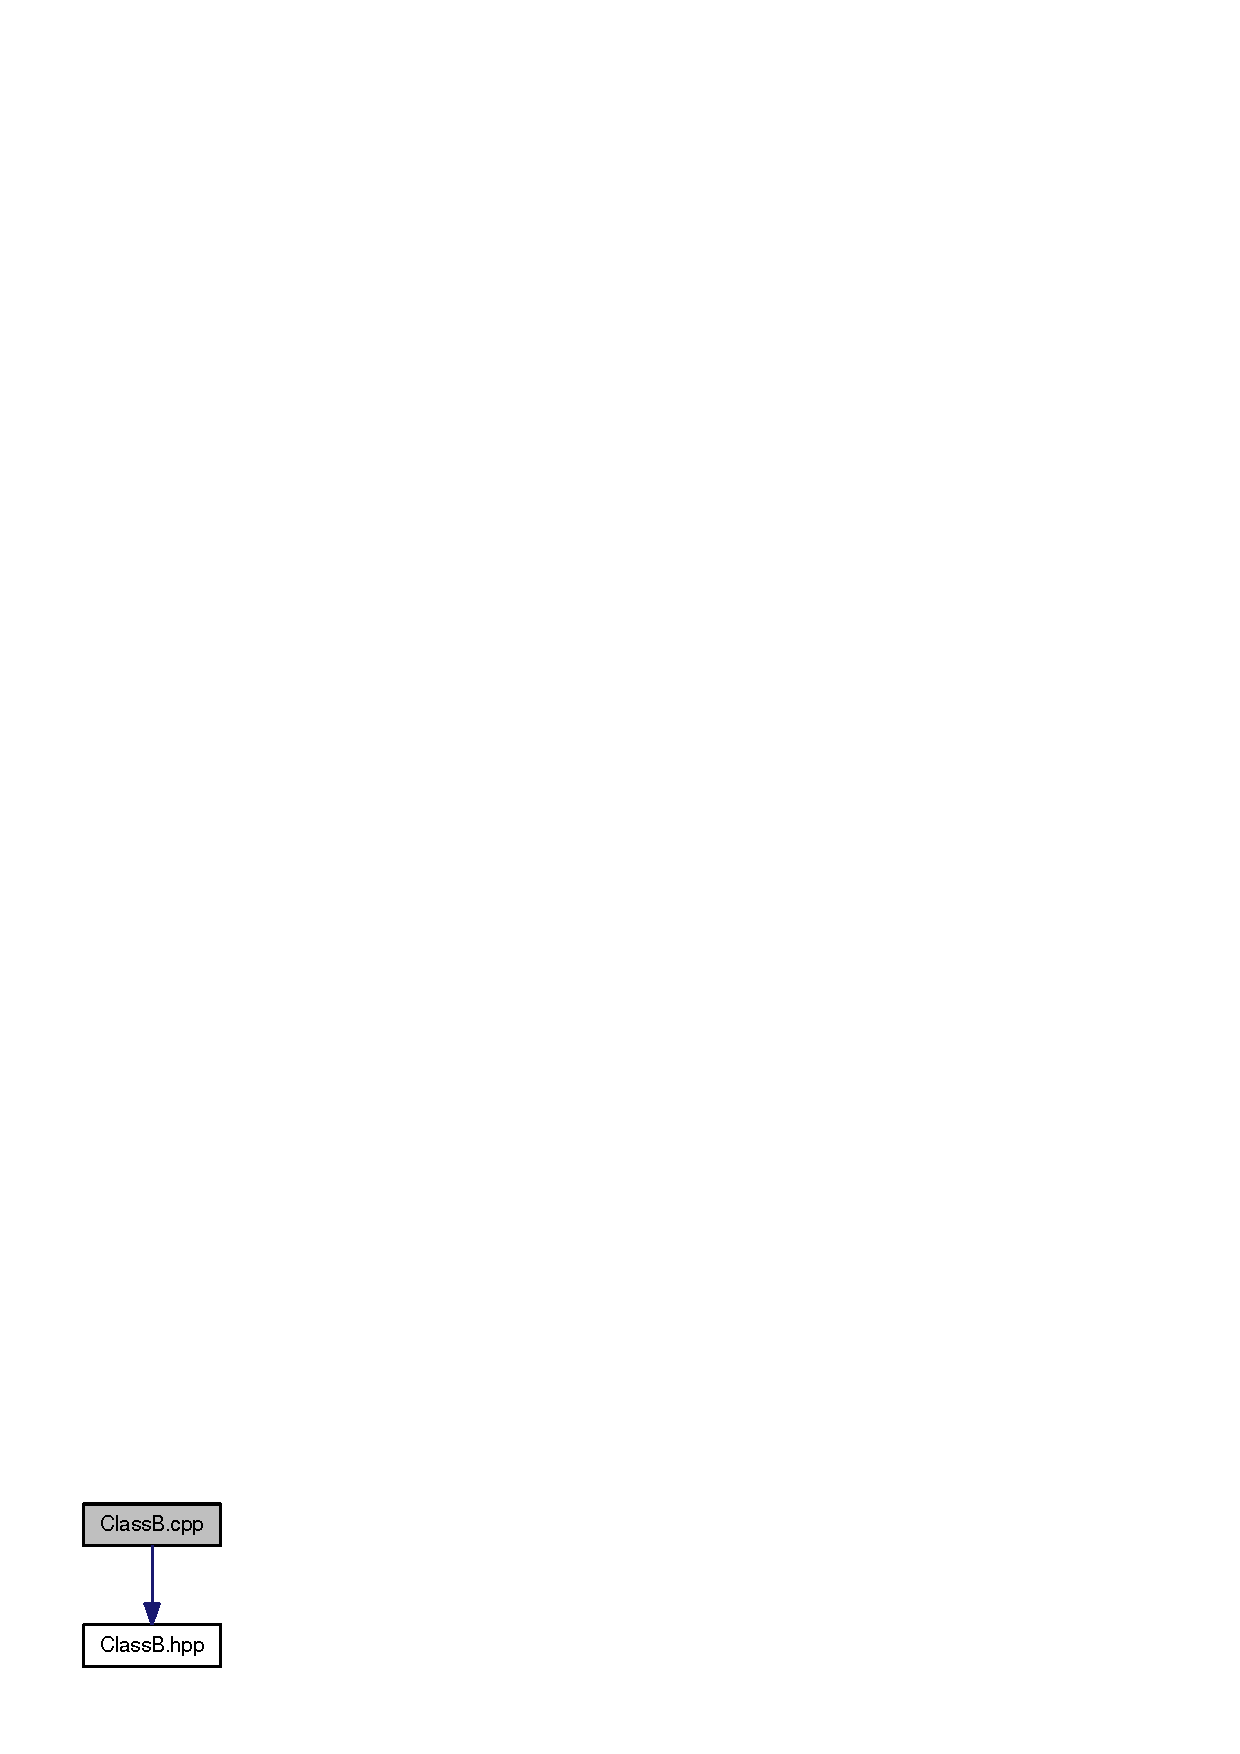
\includegraphics[width=55pt]{_class_b_8cpp__incl}
\end{center}
\end{figure}

\hypertarget{_class_b_8hpp}{
\section{Référence du fichier ClassB.hpp}
\label{_class_b_8hpp}\index{ClassB.hpp@{ClassB.hpp}}
}
Ce graphe montre quels fichiers incluent directement ou indirectement ce fichier :\nopagebreak
\begin{figure}[H]
\begin{center}
\leavevmode
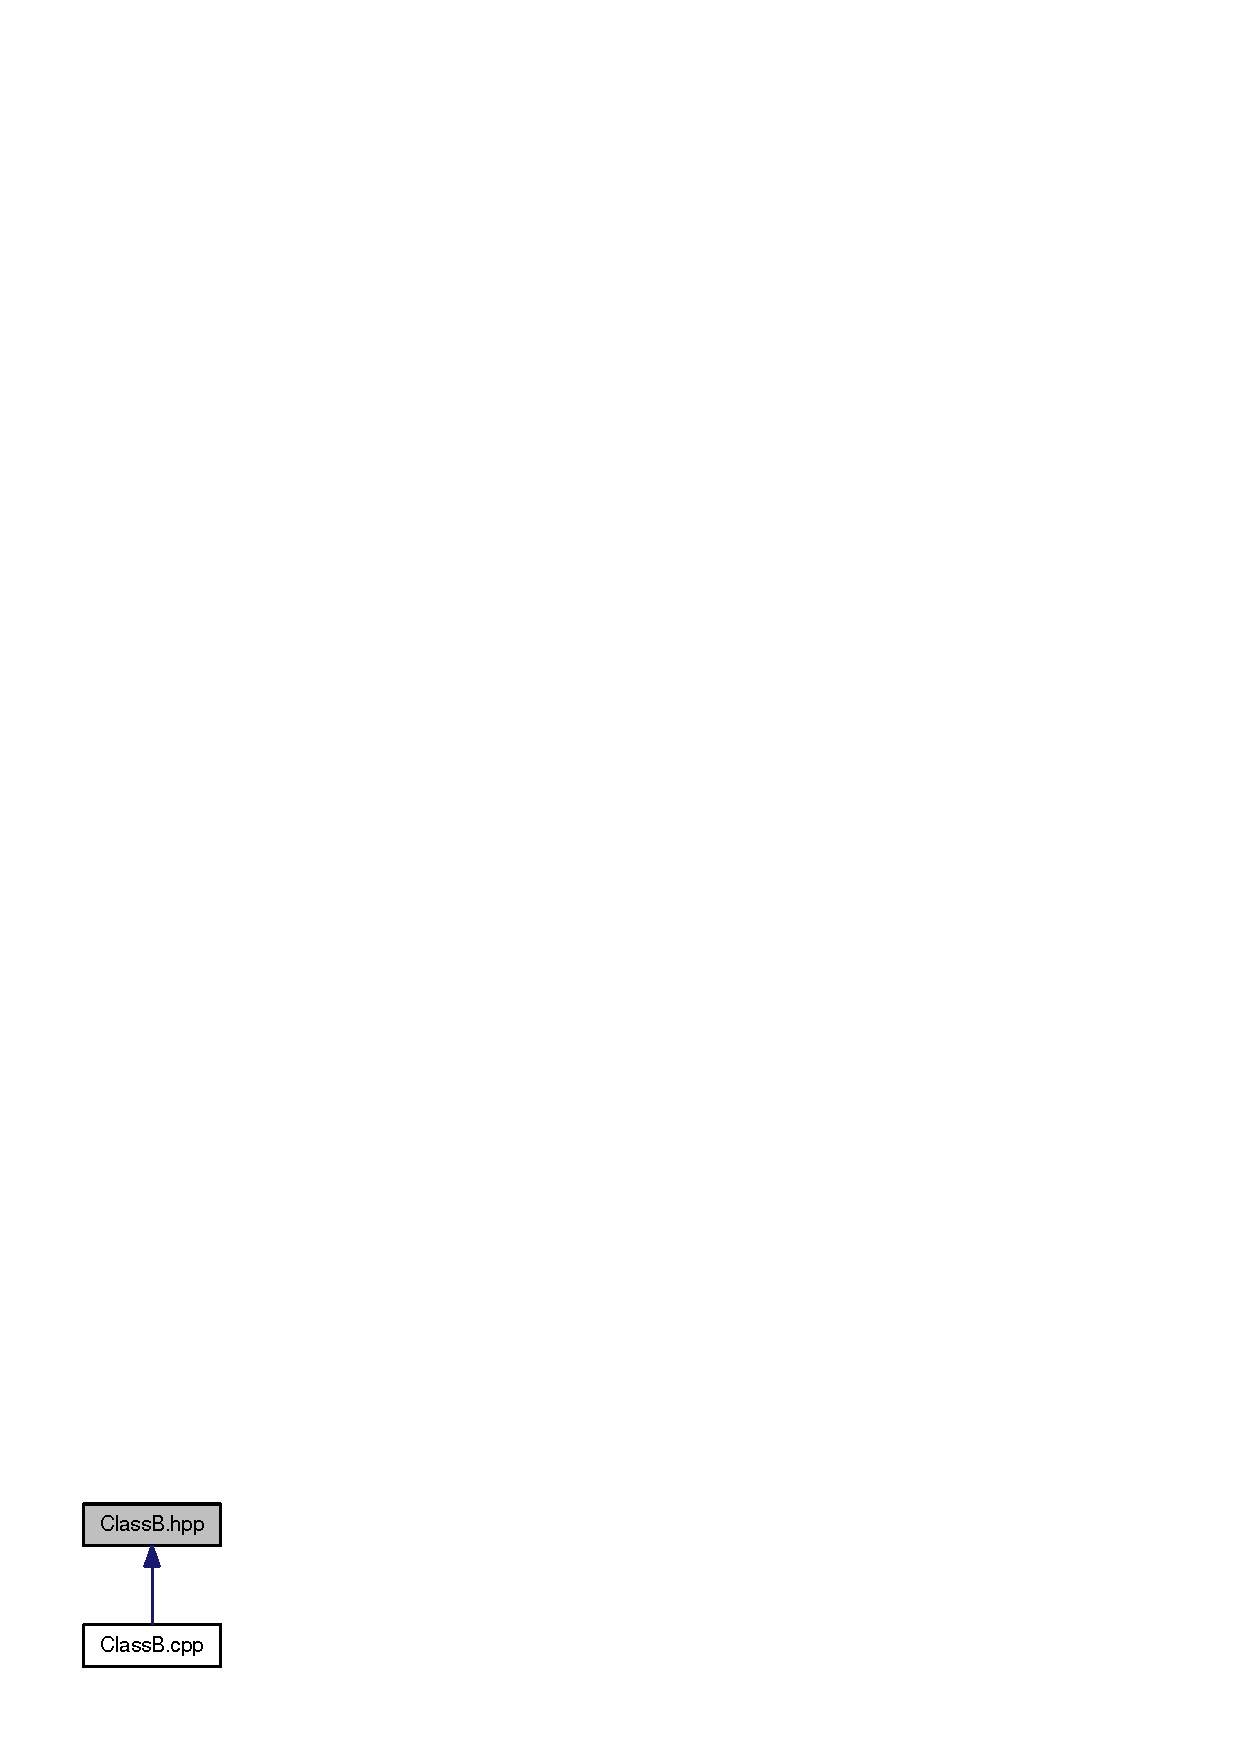
\includegraphics[width=55pt]{_class_b_8hpp__dep__incl}
\end{center}
\end{figure}
\subsection*{Classes}
\begin{DoxyCompactItemize}
\item 
class \hyperlink{class_class_b}{ClassB}
\begin{DoxyCompactList}\small\item\em Classe d'exemple B. \item\end{DoxyCompactList}\end{DoxyCompactItemize}


\subsection{Description détaillée}

\printindex
\end{document}
